
\documentclass[10pt,a4paper]{report}
%\usepackage[latin1]{inputenc}
\usepackage[utf8]{inputenc}
\usepackage{amsmath}
\usepackage{amsfonts}
\usepackage{amssymb}
\usepackage{graphicx}
\usepackage{multicol}
\usepackage{tabularx}
\usepackage{tikz}
\usetikzlibrary{arrows,shapes,automata,petri,positioning,calc}
\usepackage{hyperref}
\usepackage{tikz}
\usetikzlibrary{matrix,calc}
\usepackage[margin=0.5in]{geometry}
\providecommand{\norm}[1]{\left\lVert#1\right\rVert}
\newcommand{\myvec}[1]{\ensuremath{\begin{pmatrix}#1\end{pmatrix}}}
\let\vec\mathbf

\newcommand{\mydet}[1]{\ensuremath{\begin{vmatrix}#1\end{vmatrix}}}

%\newcommand{\myvec}[1]{\ensuremath{\begin{pmatrix}#1\end{pmatrix}}}
%\let\vec\mathbf
\providecommand{\mtx}[1]{\mathbf{#1}}
\newenvironment{Figure}
  {\par\medskip\noindent\minipage{\linewidth}}
  {\endminipage\par\medskip}
\begin{document}
%--------------------logo figure-------------------------%
\begin{figure*}[!tbp]
  \centering
  \begin{minipage}[b]{0.4\textwidth}
   
\includegraphics[scale=0.05]{/sdcard/Download/FWC-main/iitlogo.jpg} 
  \end{minipage}
  \hfill
  \vspace{5mm}\begin{minipage}[b]{0.4\textwidth}
\raggedleft 
\includegraphics[scale=0.1]{/sdcard/Download/FWC-main/nrc.jpeg} 

  \end{minipage}\vspace{0.2cm}
\end{figure*}
%--------------------name & rollno-----------------------
\raggedright \textbf{Name}:\hspace{1mm}Prathyusha Korepu\hspace{3cm} \Large \textbf{Line Assignment}\hspace{2.5cm} % 
\normalsize \textbf{Roll No.} :\hspace{1mm} FWC22047\vspace{1cm}
\begin{multicols}{2}


%----------------problem statement--------------%
\raggedright \textbf{Problem Statement:}\vspace{2mm}
\raggedright \\The x-coordinate of the incentre of the triangle that has the
coordinates of mid points of its sides as (0, 1)(1, 1)and (1,0) is:

(a)2+$\sqrt{2}$  \hspace{2cm} (b)2-$\sqrt{2}$ 

(c)1+$\sqrt{2}$ \hspace{2cm}  (d)1-$\sqrt{2}$\\
\vspace{5mm}
 \vspace{2mm} 
 \textbf{Construction}
\begin{center}
\setlength{\arrayrulewidth}{0.5mm}
\setlength{\tabcolsep}{6pt}
\renewcommand{\arraystretch}{1.5}
    \begin{tabular}{|l|c|}
    \hline 
    \textbf{vertex} & \textbf{coordinates} \\ \hline
  
   P & $ \begin{pmatrix} 
1 \\
0
\end{pmatrix} $ \\ \hline  
   Q & $ \begin{pmatrix} 
0 \\
1
\end{pmatrix} $ \\ \hline
   R & $ \begin{pmatrix} 
1\\
1
\end{pmatrix} $ \\ \hline
k&1\\   \hline
	A& $ \begin{pmatrix} 
0\\
0
\end{pmatrix} $ \\
 \hline
	B & $ \begin{pmatrix} 
2\\
0
\end{pmatrix} $ \\
\hline
 C & $ \begin{pmatrix} 
0 \\
2
\end{pmatrix} $ \\ \hline
      \end{tabular}
  \end{center}

\textbf{Solution:}
If a point P divides the line segment AB in the ratio 1: 1 is given by
\vspace{2mm}
\begin{equation*}
P= \frac{B+A}{2}
\end{equation*}\\
\begin{equation*}
 A+B=2P
\end{equation*} \\

\begin{center}


$ \begin{pmatrix} 
A
B
C
\end{pmatrix} $ 
$ \begin{pmatrix} 
1 \\
1 \\
0
\end{pmatrix} $ =2P\\
\end{center}
\vspace{3mm}
\begin{equation*}
R=\frac{B+C}{2}
\end{equation*} \\
\begin{equation*}
B+C=2R
\end{equation*} \\
\begin{center}
$ \begin{pmatrix} 
A
B
C
\end{pmatrix} $ 
$ \begin{pmatrix} 
0 \\
1 \\
1
\end{pmatrix} $ =2R\\
\end{center}
\begin{equation*}
Q=\frac{A+C}{2}
\end{equation*} \\
\begin{equation*}
A+C=2Q
\end{equation*} \\
\begin{center}
$ \begin{pmatrix} 
A
B
C
\end{pmatrix} $ 
$ \begin{pmatrix} 
1 \\
0 \\
1
\end{pmatrix} $ =2Q\\
\end{center}
\begin{center}
$ \begin{pmatrix} 
A
B
C
\end{pmatrix} $ 
$ \begin{pmatrix} 
1 & 1 & 0 \\
1 & 0 & 1 \\
0 & 1 & 1
\end{pmatrix} $ =2$ \begin{pmatrix} 
P 
Q
R
\end{pmatrix} $ \\
\end{center}
\begin{center}
$ \begin{pmatrix} 
A
B
C
\end{pmatrix} $ 
V=2$ \begin{pmatrix} 
P 
Q 
R
\end{pmatrix} $ \\
\end{center}
\begin{center}
$ \begin{pmatrix} 
A
B
C
\end{pmatrix} $ 
=2$ \begin{pmatrix} 
P 
Q 
R
\end{pmatrix} $ 
$\vec{V}^{-1}$\\
\end{center}
\begin{center}
$\vec{V}^{-1}$=$\frac{-1}{2}$
$ \begin{pmatrix} 
-1 & -1 & 1 \\
-1 & 1 & -1 \\
1 & -1 & -1
\end{pmatrix} $ \\
\end{center}
\begin{center}
$ \begin{pmatrix} 
A
B
C
\end{pmatrix} $ 
	=2($\frac{-1}{2}$) $ \begin{pmatrix} 
P 
Q 
R
\end{pmatrix} $ 
$ \begin{pmatrix} 
-1 & -1 & 1 \\
-1 & 1 & -1 \\
1 & -1 & -1
\end{pmatrix} $\\
\end{center}
\begin{center}
$ \begin{pmatrix} 
A
B
C
\end{pmatrix} $ =
$ \begin{pmatrix} 
-P-Q+R \hspace{3mm}
-P+Q-R\hspace{3mm}
P-Q-R
\end{pmatrix} $ 
\end{center}
Given P  $ \begin{pmatrix}
  1 \\
  0
 \end{pmatrix} $ \hspace{3mm}
     Q  $ \begin{pmatrix}
  0 \\
  1
  \end{pmatrix} $ \hspace{3mm}
     R  $ \begin{pmatrix}
  1\\
  1
  \end{pmatrix} $ \\
By substituting P,Q and R in above equqtion, we will get A,B and C as \\
\vspace{2mm}
 A $ \begin{pmatrix} 
0 \\
0
\end{pmatrix} $  \hspace{2mm}
B $ \begin{pmatrix} 
2 \\
0
\end{pmatrix} $  \hspace{4mm}
C $ \begin{pmatrix}
0 \\
2
\end{pmatrix} $  \\ 
\vspace{2mm}
Vector representation of A,B,C are as follows
\begin{equation}
\vec{A=0}
\end{equation}\\
\begin{equation}
\vec{B=2i}
\end{equation}\\
\begin{equation}
\vec{C=2j}
\end{equation}\\
The vectors of AB,BC and CA linesegments are   \\
\begin{equation}
\vec{V1   = B-A=2i}
\end{equation}\\
\begin{equation}
\vec{V2 = C-B=2j-2i}
\end{equation}\\
\begin{equation}
\vec{V3 = A-C=-2j}
\end{equation} \\
Norms of the vectors V1, V2 and V3 are 

 
\begin{align}
\norm{\vec{V1}}=2
\end{align}

\begin{align}
{\norm{\vec{V2}}}=2\sqrt{2} 
\end{align}
\begin{align}
\norm{\vec{V3}}=2
\end{align}



The incenter is the intersection of three angle bisectors,

\begin{align}
I=\frac{\norm{\vec{V1}}{\vec{C}}+\norm{\vec{V2}}{\vec{A}}+\norm{\vec{V3}}{\vec{B}}}{\norm{\vec{V1}}+\norm{\vec{V2}}+\norm{\vec{V3}}}
\end{align}
\begin{align*}
I=\frac{2({\vec{2i}})+2({\vec{2j}})+2\sqrt{2}({\vec{0}})}{2+2+2\sqrt{2}}
\end{align*}
\begin{align*}
I=\frac{\vec{4i+4j}}{4+2\sqrt{2}}
\end{align*}	 
The x-coordinate of the incentre of the triangle is
\begin{align*}
x=\frac{\vec{4i}}{4+2\sqrt{2}}
\end{align*}	 
\begin{equation}
x=2-\sqrt{2}
\end{equation}
\begin{center}
 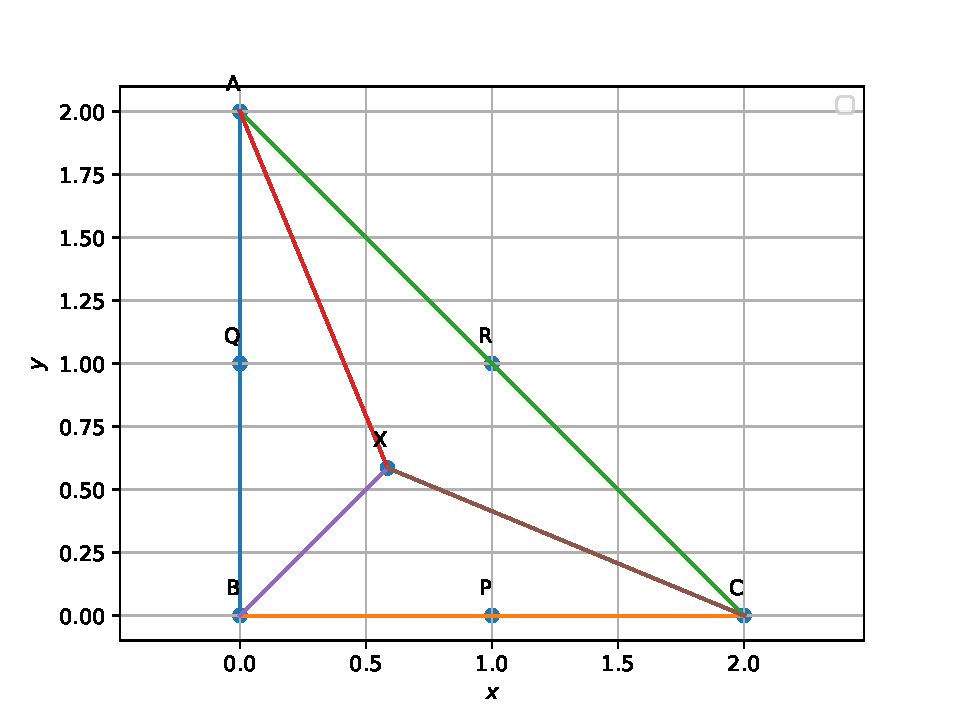
\includegraphics[scale=0.5]{/sdcard/Download/FWC-main/FWC-main/matrix/line_fig.pdf}  
 \end{center} 
 
\raggedright  Download the code from  
Github link: \href{https://github.com/Prathyushakorepu/FWC/tree/main/Matrix/Line_assignment}{Assignment-4}.
  \end{multicols}
\end{document}
